% Template laporan ini dibuat dengan harapan untuk standardisasi laporan praktikum pada lingkungan DTEDI SV UGM, agar semua laporan praktikum konsisten secara format dan hasil cetak laporan.
% Saran dan perbaikan sangat diperlukan agar template ini dapat digunakan oleh semua orang. bila ada saran, silahkan hubungi author melalui linkedin : Alim Satria
% Dibuat oleh : Alim Satria Fi'i Wijaya Kusuma

\documentclass[12 pt]{article}
\usepackage[a4paper, total={6in, 9in}]{geometry}
\usepackage[utf8]{inputenc}
\usepackage{color}
\usepackage[bahasa]{babel}
\usepackage{float}
\usepackage{graphicx}
\usepackage{amsmath}
\usepackage{setspace}
\usepackage{indentfirst}

\renewcommand \thesection{\Roman{section}.}
\renewcommand \thesubsection{\arabic{section}.\arabic{subsection}.}
\renewcommand \figurename{Gambar}
\renewcommand \thefigure {\arabic{section}.\arabic{subsection}.\arabic{figure} } %kustom nomor gambar dengan format (section.subsection.urutan_figure)
\renewcommand \tablename{Tabel}
\renewcommand \thetable {\arabic{section}.\arabic{subsection}.\arabic{table} } %kustom nomor tabel dengan format (section.subsection.urutan_tabel)
\renewcommand \theequation{\arabic{section}.\arabic{equation}} %kustom pemomoran persamaan matematika (section.urutan_persamaan)
\setlength{\tabcolsep}{10pt} %kustom spacing coloumn tabel (default = 6pt)
\renewcommand{\arraystretch}{1.5} %kustom spacing row tabel (default = 1)

\title{\large \textbf{LAPORAN [MATA-KULIAH-PRAKTIKUM]} \\ \textbf{[JUDUL-PRAKTIKUM]}\linebreak}
\author{}
\date{}
\onehalfspacing

\begin{document}

\clearpage
\maketitle
\thispagestyle{empty} %menghapus penomoran pada cover

\begin{center}

\includegraphics[width=5cm,height=5cm]{cover_laporan/logo_ugm.png}
\end{center}

\vspace{1 cm}

\begin{center}
\begin{tabular}{lcl}
Nama & : & Nama-Praktikan \\
NIM & : & NIM-Praktikan\\
Kelas & : & Kelas-Praktikum\\
Tanggal & : & Tanggal-Praktikum
\end{tabular}
\newline
\newline
\newline
\newline
\newline
\large{\textbf{PROGRAM STUDI TEKNOLOGI REKAYASA INSTRUMENTASI DAN KONTROL}} \\
\textbf{SEKOLAH VOKASI UNIVERSITAS GADJAH MADA} \\
\textbf{2022}
\end{center}

\pagebreak

\section{Dasar Teori}

Lorem ipsum dolor sit amet, consectetur adipiscing elit. Suspendisse nec enim eu neque blandit pulvinar nec ut orci. In id diam non lorem gravida porta facilisis nec elit. Duis non vehicula erat, eu volutpat nisl. Sed ultricies odio sit amet massa lacinia, a gravida metus ultrices. Proin vestibulum, ipsum interdum maximus malesuada, risus libero scelerisque urna, sit amet semper purus est at ex. Praesent mollis odio eu dictum pretium. Donec et diam varius neque gravida fringilla sed in velit. Quisque pretium metus at erat feugiat, eu viverra velit rutrum. Suspendisse ac libero velit. Morbi molestie dui vitae eleifend venenatis. Nam viverra felis nisl, et maximus lorem lobortis vitae. Lorem ipsum dolor sit amet, consectetur adipiscing elit. Donec felis lorem, volutpat sit amet nisi ac, sagittis sodales justo. Fusce euismod auctor fermentum. Nullam aliquam condimentum nisi, vitae blandit erat fermentum ut.

\begin{figure}[H]
    \centering
    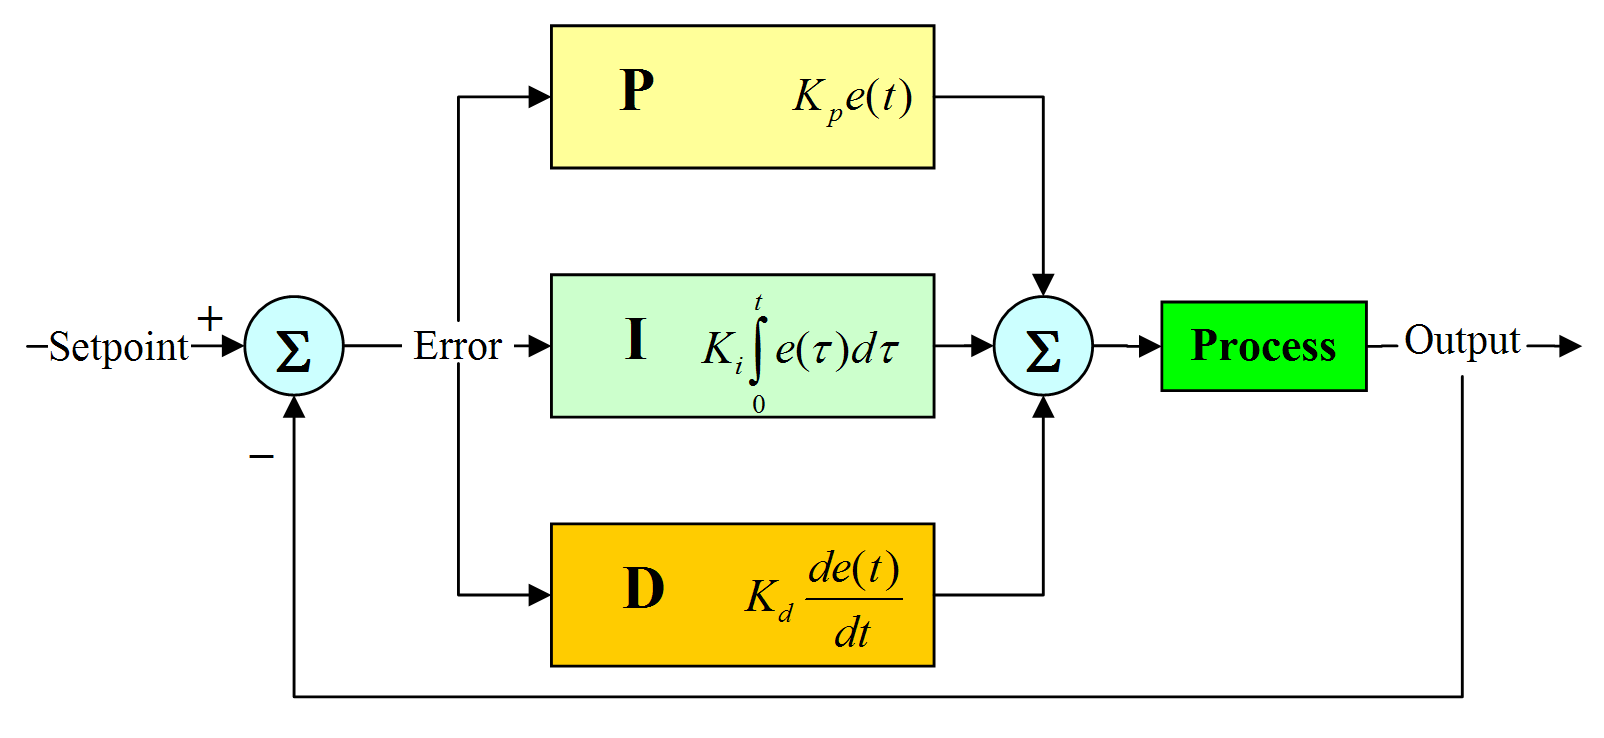
\includegraphics[width = \textwidth]{gambar_praktikum/gambar_pid.png}
    \caption{ini-contoh-gambar}
    \label{ini-label-gambar}
\end{figure}

Seperti yang ditunjukkan Gambar \ref{ini-label-gambar} yang merupakan contoh penggunaan referensi gambar pada \LaTeX, Pellentesque viverra interdum luctus. Vestibulum et mi molestie metus tempor aliquam. Nulla porttitor mi a odio commodo, eget molestie justo pulvinar. Sed sit amet justo sagittis, lobortis erat eu, pharetra nulla. Sed fermentum ex quis venenatis fermentum. Sed metus neque, sollicitudin sed metus vel, pellentesque feugiat lorem. Curabitur ipsum nibh, convallis tincidunt augue non, euismod hendrerit libero. Nullam sed ante sit amet mauris sodales dictum ut id leo. Aenean eget felis malesuada, facilisis ante et, feugiat eros. Cras eu pellentesque ex. Aenean mollis consequat nisi ac congue. Sed non orci mauris.

\section{Alat dan Bahan Praktikum}

Alat dan bahan praktikum dapat disebutkan sebagaimana berikut,

\begin{table}[H]
\centering
\begin{tabular}{lll}
\hline
\multicolumn{1}{c}{No.} & \multicolumn{1}{c}{Nama Alat} & \multicolumn{1}{c}{Jumah alat} \\ \hline
1.                      & Arduino Uno                   & 1 Pcs                          \\
2.                      & Kabel Jumper                  & 3 Pcs                          \\
3.                      & Bread Board                   & 1 Pcs                          \\
4.                      & LED                           & 2 Pcs                         
\end{tabular}
\end{table}


\section{Langkah Praktikum}

\subsection{Langkah Praktikum Pertama}

Langkah praktikum dapat dibuat sebagaimana berikut,

\begin{enumerate}
    \item Ini langkah pertama
    \item Ini langkah kedua
    \item Dan seterusnya...
\end{enumerate}

\subsection{Langkah Praktikum Kedua}

Langkah praktikum dapat dibuat sebagaimana berikut,

\begin{enumerate}
    \item Ini langkah pertama
    \item Ini langkah kedua
    \item Dan seterusnya...
\end{enumerate}

\section{Hasil dan Pembahasan}

\subsection{Hasil Percobaan Satu}

Berikut merupakan contoh membuat persamaan matematika pada \LaTeX,
    
\begin{equation}
\label{persamaan_percobaan_satu}
    a = b + c
\end{equation}

Seperti yang dijelaskan Persamaan \eqref{persamaan_percobaan_satu}, yang merupakan cara untuk membuat referensi persamaan dengan \LaTeX. Begitupun dengan Persamaan \eqref{persamaan_percobaan_dua}

\begin{equation}
    \label{persamaan_percobaan_dua}
    I = \frac{V}{R}
\end{equation}

\subsection{Hasil Percobaan Dua}

\section{Kesimpulan}

\end{document}